% 17-71(17쪽) — 반지름 2 인 원 O 와 그 위의 점 A 를 중심으로 한 반지름 r 인 원, 두 원의 교점 P·Q, 지름 AB 와 만나는 점 R, 색칠한 사각형 APRQ. 스캔 화질이 낮아 TikZ 로 다시 그림.
% 원문 라벨(A·B·O·P·Q·R·파선 r·파선 2)만 옮긴다. r 는 0<r<4 의 일반 위치라 답(r→4− 극한)이 그림에서 읽히지 않는다.
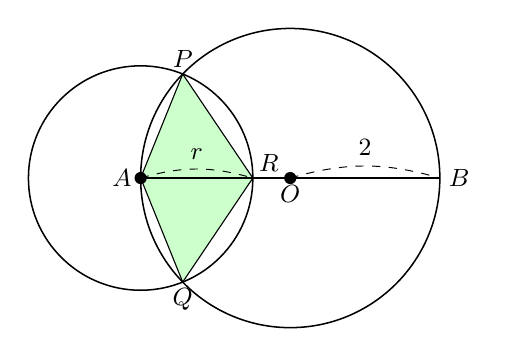
\begin{tikzpicture}[x=0.95cm, y=0.95cm, line width=0.6pt]
  \fill[green!20] (-2,0) -- (-1.4375,1.3905) -- (-0.5,0) -- (-1.4375,-1.3905) -- cycle;
  \draw[line width=0.4pt] (-2,0) -- (-1.4375,1.3905) -- (-0.5,0) -- (-1.4375,-1.3905) -- cycle;
  \draw[line width=0.55pt] (0,0) circle (2);
  \draw[line width=0.55pt] (-2,0) circle (1.5);
  \draw[line width=0.5pt] (-2,0) -- (2,0);
  \draw[dashed, line width=0.35pt] (-2,0) to[bend left=16] (-0.5,0);
  \draw[dashed, line width=0.35pt] (0,0) to[bend left=16] (2,0);
  \fill (-2,0) circle (2.2pt);
  \fill (0,0) circle (2.2pt);
  \node[font=\small, inner sep=3pt, left] at (-2,0) {$\pt{A}$};
  \node[font=\small, inner sep=3pt, right] at (2,0) {$\pt{B}$};
  \node[font=\small, inner sep=2.5pt, below] at (0,0) {$\pt{O}$};
  \node[font=\small, inner sep=2pt, above right] at (-0.5,0) {$\pt{R}$};
  \node[font=\small, inner sep=1.5pt, above] at (-1.25,0.18) {$r$};
  \node[font=\small, inner sep=1.5pt, above] at (1.0,0.24) {$2$};
  \node[font=\small, inner sep=2pt, above] at (-1.4375,1.3905) {$\pt{P}$};
  \node[font=\small, inner sep=2pt, below] at (-1.4375,-1.3905) {$\pt{Q}$};
\end{tikzpicture}
